\documentclass[tikz,border=12pt]{standalone}
\usepackage[T1]{fontenc}
\usepackage{mathpazo}
\usepackage{amsmath,amssymb}
\usetikzlibrary{arrows.meta, positioning, calc, decorations.pathreplacing}

\definecolor{stblue}{HTML}{7B97AD}
\definecolor{rwgold}{HTML}{B8995E}
\definecolor{sage}{HTML}{7A9A7E}
\definecolor{dkbrown}{HTML}{3D3530}
\definecolor{wmgray}{HTML}{7B7067}
\definecolor{cream}{HTML}{F9F6F0}
\definecolor{border}{HTML}{D4C9B8}
\definecolor{terracotta}{HTML}{C47A6A}

\begin{document}
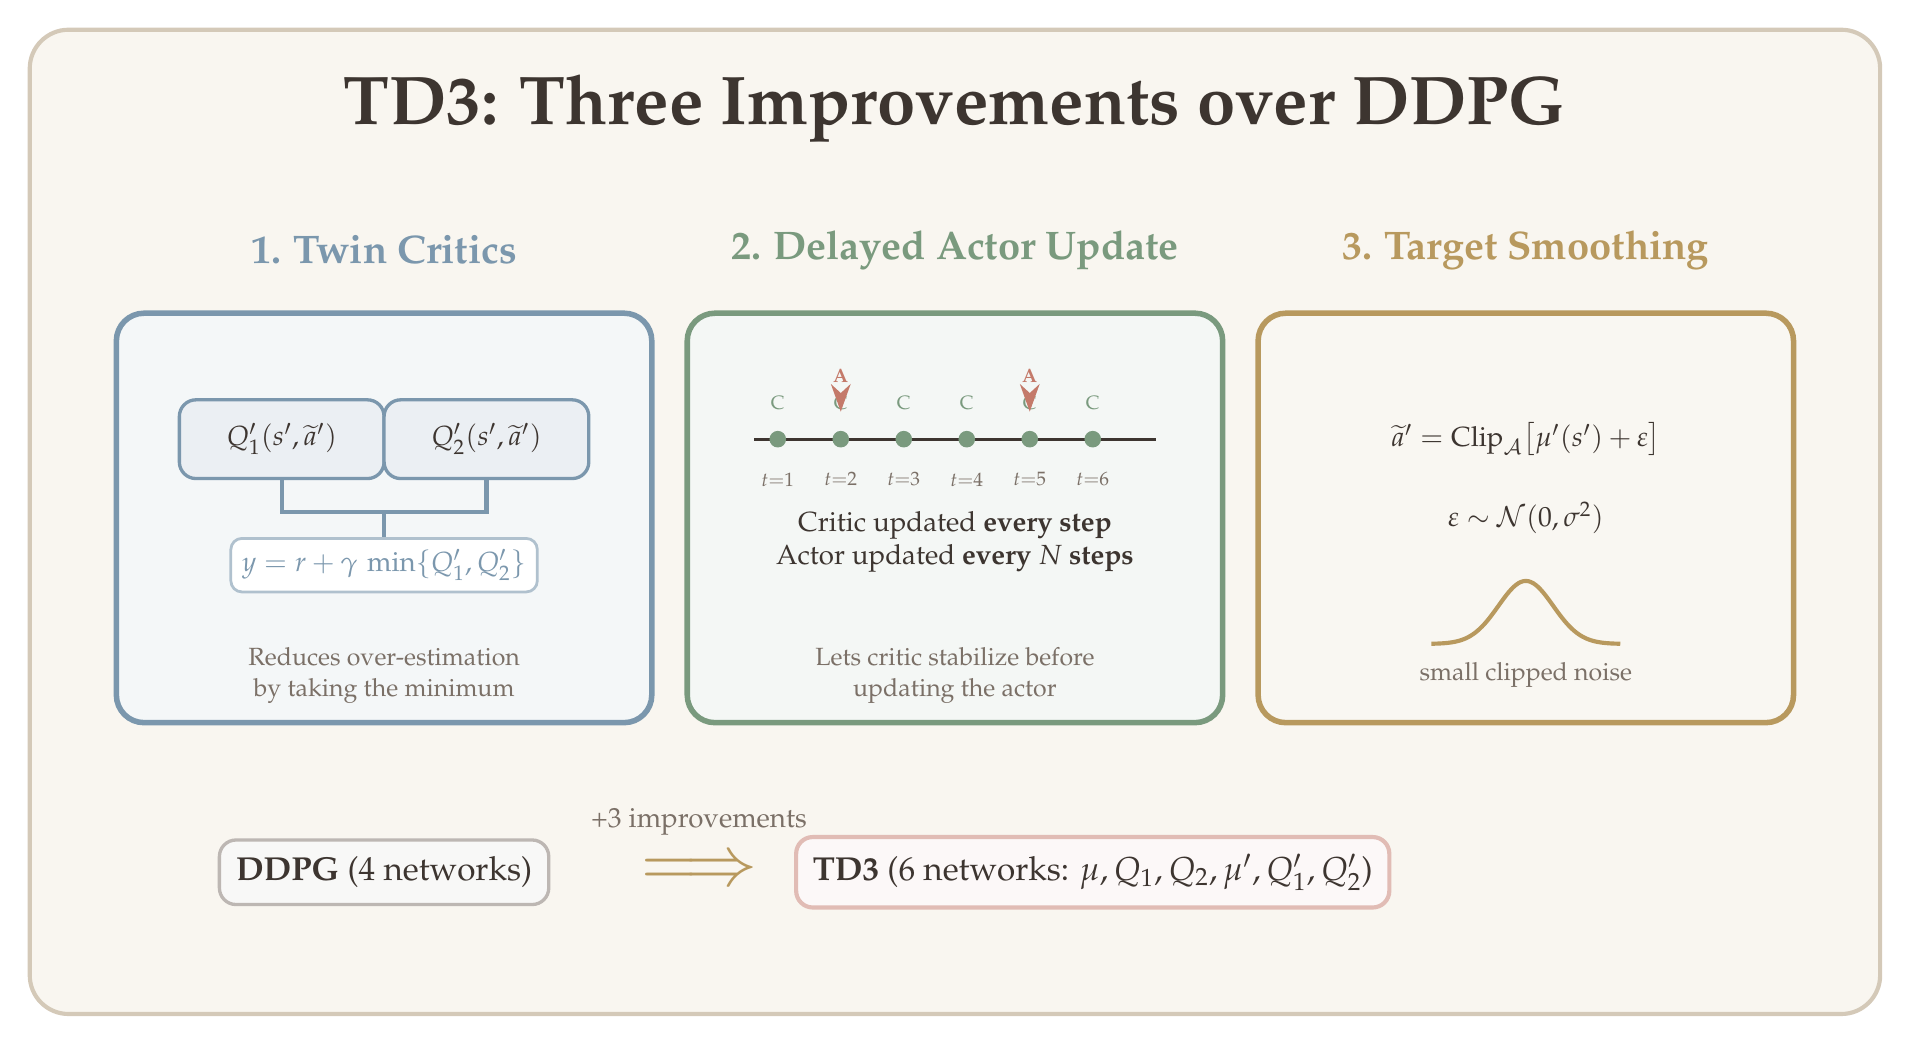
\begin{tikzpicture}[
  >={Stealth[length=3.5mm, width=2.5mm]},
  impbox/.style={
    draw=#1, line width=2pt, fill=#1!8, rounded corners=10pt,
    minimum width=68mm, minimum height=52mm, font=\large, text=dkbrown,
    align=center, inner sep=8pt
  },
  lbl/.style={font=\normalsize, text=wmgray, align=center},
]

% Background
\fill[cream, rounded corners=14pt] (-1,-1.5) rectangle (22.5,11);
\draw[border, rounded corners=14pt, line width=1.5pt] (-1,-1.5) rectangle (22.5,11);

% Title
\node[font=\Huge\bfseries, text=dkbrown] at (10.75,10)
  {TD3: Three Improvements over DDPG};

% =============================================
% Improvement 1: Twin Critics
% =============================================
\node[impbox=stblue] (twin) at (3.5,4.8) {};
\node[font=\Large\bfseries, text=stblue] at (3.5,8.2) {1. Twin Critics};

% Two critic boxes inside
\node[draw=stblue, line width=1.2pt, fill=stblue!15, rounded corners=6pt,
      minimum width=26mm, minimum height=10mm, font=\normalsize, text=dkbrown]
  (q1) at (2.2,5.8) {$Q_1'(s', \widetilde{a}')$};
\node[draw=stblue, line width=1.2pt, fill=stblue!15, rounded corners=6pt,
      minimum width=26mm, minimum height=10mm, font=\normalsize, text=dkbrown]
  (q2) at (4.8,5.8) {$Q_2'(s', \widetilde{a}')$};

% Min arrow
\draw[->, line width=1.5pt, stblue] (q1.south) -- ++(0,-0.4) -| (3.5,4.2);
\draw[->, line width=1.5pt, stblue] (q2.south) -- ++(0,-0.4) -| (3.5,4.2);
\node[draw=stblue!60, line width=1pt, fill=white, rounded corners=4pt,
      font=\normalsize\bfseries, text=stblue, inner sep=4pt]
  at (3.5,4.2) {$y = r + \gamma\,\min\{Q_1', Q_2'\}$};

% Description
\node[font=\small, text=wmgray, align=center] at (3.5,2.8)
  {Reduces over-estimation\\by taking the minimum};

% =============================================
% Improvement 2: Delayed Actor Update
% =============================================
\node[impbox=sage] (delay) at (10.75,4.8) {};
\node[font=\Large\bfseries, text=sage] at (10.75,8.2) {2. Delayed Actor Update};

% Timeline
\draw[dkbrown, line width=1pt] (8.2,5.8) -- (13.3,5.8);
\foreach \x/\t in {8.5/1, 9.3/2, 10.1/3, 10.9/4, 11.7/5, 12.5/6} {
  \fill[sage] (\x, 5.8) circle (3pt);
  \node[font=\scriptsize, text=wmgray, below] at (\x, 5.5) {$t{=}\t$};
}
% Critic updates (every step)
\foreach \x in {8.5, 9.3, 10.1, 10.9, 11.7, 12.5} {
  \node[font=\scriptsize, text=sage, above] at (\x, 6.05) {C};
}
% Actor updates (every N steps)
\foreach \x in {9.3, 11.7} {
  \node[font=\scriptsize\bfseries, text=terracotta, above] at (\x, 6.4) {A};
  \draw[terracotta, line width=1pt, ->] (\x, 6.35) -- (\x, 6.15);
}

% Description
\node[font=\normalsize, text=dkbrown, align=center] at (10.75,4.5)
  {Critic updated \textbf{every step}\\Actor updated \textbf{every $N$ steps}};
\node[font=\small, text=wmgray, align=center] at (10.75,2.8)
  {Lets critic stabilize before\\updating the actor};

% =============================================
% Improvement 3: Target Policy Smoothing
% =============================================
\node[impbox=rwgold] (smooth) at (18,4.8) {};
\node[font=\Large\bfseries, text=rwgold] at (18,8.2) {3. Target Smoothing};

% Equation
\node[font=\normalsize, text=dkbrown, align=center] at (18,5.8)
  {$\widetilde{a}' = \text{Clip}_{\mathcal{A}}\bigl[\mu'(s') + \varepsilon\bigr]$};
\node[font=\normalsize, text=dkbrown, align=center] at (18,4.8)
  {$\varepsilon \sim \mathcal{N}(0, \sigma^2)$};

% Noise illustration
\draw[rwgold, line width=1.5pt, smooth] plot[domain=-1.2:1.2, samples=40]
  ({18 + \x}, {3.2 + 0.8*exp(-(\x)^2/(2*0.12))});
\node[font=\small, text=wmgray] at (18,2.8) {small clipped noise};

% =============================================
% Bottom: DDPG -> TD3 progression
% =============================================
\node[draw=wmgray!50, line width=1.2pt, fill=wmgray!5, rounded corners=6pt,
      font=\large, text=dkbrown, inner sep=6pt]
  (ddpg-box) at (3.5,0.3) {\textbf{DDPG} (4 networks)};
\node[font=\Huge, text=rwgold] at (7.5,0.3) {$\Longrightarrow$};
\node[font=\normalsize, text=wmgray, above] at (7.5,0.65) {+3 improvements};
\node[draw=terracotta!50, line width=1.5pt, fill=terracotta!5, rounded corners=6pt,
      font=\large, text=dkbrown, inner sep=6pt]
  (td3-box) at (12.5,0.3) {\textbf{TD3} (6 networks: $\mu, Q_1, Q_2, \mu', Q_1', Q_2'$)};

\end{tikzpicture}
\end{document}
